\documentclass{article}
\usepackage{tikz}
\usetikzlibrary{arrows,decorations.pathmorphing,backgrounds,positioning,fit,petri,automata}

% Custom styles for number line
\tikzset{
    mylabel/.style={font=\footnotesize},
    numberline/.style={thin, black},
    tick/.style={black, thin, opacity=1},
    point/.style={black, thick},
}

\begin{document}

\begin{tikzpicture}
    % Draw the number line
    \draw[<->] (-3,0) -- (3,0);

    % Draw the ticks and labels
    \foreach \x in {-2,-1,0,1,2}
    \draw (\x, 0.1) -- (\x, -0.1) node[below] {\x};

    % Mark a specific point (optional)
    \draw[fill=black] (1,0) circle (2pt) node[above=5pt] {1};
\end{tikzpicture}


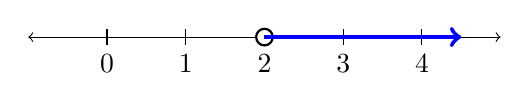
\begin{tikzpicture}
    % Draw the number line
    \draw[<->] (-1,0) -- (5,0);
    \foreach \x in {0,1,2,3,4}
    \draw (\x, 0.1) -- (\x, -0.1) node[below] {\x};

    % Draw the open circle at the endpoint
    \draw[fill=white, thick] (2,0) circle (3pt);

    % Draw the line extending from the circle
    \draw[ultra thick, blue, ->] (2,0) -- (4.5,0);
\end{tikzpicture}

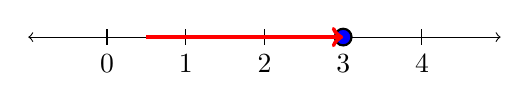
\begin{tikzpicture}
    % Draw the number line
    \draw[<->] (-1,0) -- (5,0);
    \foreach \x in {0,1,2,3,4}
    \draw (\x, 0.1) -- (\x, -0.1) node[below] {\x};

    % Draw the filled circle at the endpoint
    \draw[fill=blue, thick] (3,0) circle (3pt);

    % Draw the line extending from the circle
    \draw[ultra thick, red, <-] (3,0) -- (0.5,0);
\end{tikzpicture}

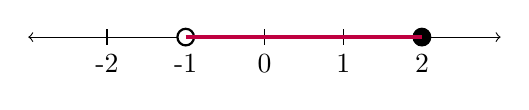
\begin{tikzpicture}
    % Draw the number line
    \draw[<->] (-3,0) -- (3,0);
    \foreach \x in {-2,-1,0,1,2}
    \draw (\x, 0.1) -- (\x, -0.1) node[below] {\x};

    % Draw the open circle at -1
    \draw[fill=white, thick] (-1,0) circle (3pt);
    % Draw the closed circle at 2
    \draw[fill=black, thick] (2,0) circle (3pt);

    % Draw the line segment between the two points
    \draw[ultra thick, purple] (-1,0) -- (2,0);
\end{tikzpicture}
    
\end{document}